\part{Applications and Algorithms}
\chapter{Superdense Coding}
The main question that we seek to answer in this section is that can we transmit more than a single classical bit on information using a single qubit? Intuitively it may seem so and this is infact true as we will see. However simply transferring a single qubit does not work because measurement collapses the qubit. Instead we will be using the properties of the four possible EPR pairs which we describe below.

\begin{figure}[htp]
    \centering
    \caption{The setup of superdense coding with Alice and Bob each possessing one qubit which are entangled}
    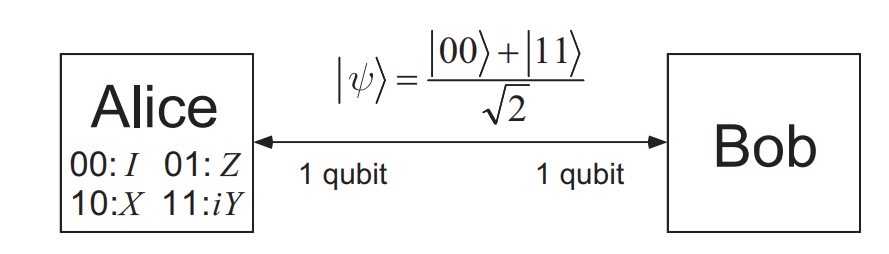
\includegraphics[width=\textwidth]{superdense}
\end{figure}

The EPR pairs or the bell states refer to the four following states comprising of two qubits that are entangled with each other.
$$ \frac{\ket{00} + \ket{11}}{\sqrt{2}}, \frac{\ket{00} - \ket{11}}{\sqrt{2}}, \frac{\ket{10} + \ket{01}}{\sqrt{2}}, \frac{\ket{01} - \ket{10}}{\sqrt{2}}$$

The main idea is that we will use the entanglement of the two qubits in one of these states to transfer two bits of information by simply transferring one bit.
Suppose Alice wants to send Bob two classical bits of information. To do so using superdense coding, an external party will first prepare the state
$$ \ket{\psi} = \frac{\ket{00} + \ket{11}}{\sqrt{2}} $$
and he will then give the first qubit to Alice and the second to Bob.
If Alice wants to send the information $00$ she will do nothing and pass her qubit to Bob.
If she wants to send $01$ then she applies the phase flip gate $Z$, if she wants to send $10$ she applies the quantum NOT gate $X$ to her qubit, if she wants to send $11$ she applies the $iY$ gate. The final state of the entangled qubits corresponding to the information she wants to send is:
$$ 00: \ket{\psi} = \frac{\ket{00} + \ket{11}}{\sqrt{2}}$$
$$ 01: \ket{\psi} = \frac{\ket{00} - \ket{11}}{\sqrt{2}} $$
$$ 10: \ket{\psi} = \frac{\ket{10} + \ket{01}}{\sqrt{2}}$$
$$ 11:  \frac{\ket{01} - \ket{10}}{\sqrt{2}} $$

Notice that all four of these states form a basis and thus when Alice passes her qubit to Bob then Bob can find out which state he got by simply measuring with respect to this basis to figure out which basis vector he had received.

\begin{exercise}
Specify which measurement operators Bob should use to figure out the two classical bits that Alice wanted to send him
\end{exercise}

Notice that this process did involve two qubits but Alice had to send only one qubit. The entanglement of the two qubits allowed Bob to figure out two classical bits of information on transfer of a single qubit.

Let's now look at the reverse, can we transmit a qubit by sending only classical information?
